\documentclass[amssymb,twocolumn,aps]{revtex4}

% allows special characters (including æøå)
\usepackage[utf8]{inputenc}
%\usepackage [norsk]{babel} %if you write norwegian
\usepackage[english]{babel}  %if you write english

\usepackage{physics,amssymb}  % mathematical symbols (physics imports amsmath)
\usepackage{graphicx}         % include graphics such as plots
\usepackage[table]{xcolor}
\usepackage{xcolor}           % set colors
\usepackage{hyperref}         % automagic cross-referencing 
\usepackage{float}			  % force placement of tables and figures
\usepackage{comment}
%\usepackage[authoryear]{natbib}


\begin{document}

\title{Report Template \\
    \normalsize FYS-STK3155 - Project X}
\date{\today}               
\author{
    Anton Nicolay Torgersen 
}
\affiliation{University of Oslo}


\newpage
    \begin{abstract}
A study of various regression methods, including OLS, Ridge and LASSO and how they fit Runge's function. 
We review the theory and implementation of these methods and see how they compare on this function.
At the end, we discuss some resampling techniques on the simpler OLS-method to understand the bias-variance trade-off.
\end{abstract}


    \maketitle
    \thispagestyle{empty} % Removes page number from the title page

    



\section{Introduction}

The fundamental problem in machine learning and statistics is to find meaningful patterns in data using models that make accurate predictions on unseen data.
This is a difficult task, as a complex function might fit the training data perfectly, but fail spectacularly when facing new instances, a phenomenon known as overfitting.
On the other hand a model that is too simple may fail to extract the patterns in the data and thus underfit the data.
Therefore understanding of the bias-variance tradeoff on simpler models before the more complex ones is paramount to develop robust and generalizable models.

Therefore, this paper will study the bias-variance tradeoff through the lens of regression models, that increase in complexity.
We start with the simplest model, Ordinary Least Squares (OLS), where we have a fully analytical solution for the best fit parameters.
Then we move on to Ridge regression, which is a regularized version of OLS, where we first introduce the tuning of a penalization parameter $\lambda$ to find a good balance between bias and variance.
Finally we end with LASSO regression, which is another regularized version of OLS, but with a different penalization term.

This analysis will closely follow the lecture notes from FYS-STK3155 \cite{compfys} and the book "The Elements of Statistical Learning" by Hastie, Tibshirani and Friedman \cite{hastie}.
We will review the theory of the three regression methods and apply the methods to a one-dimensional problem, fitting a polynomial model to Runge's function, $f(x)=1/(1+25x^2)$.
This function is notoriously difficult for high-degree polynomial interpolation and will therefore be a good demonstration of the pitfalls of overfitting and the benefits of regularized techniques like Ridge and LASSO.
Together these three models will create a better understanding of the dynamics between bias and variance, how the dynamic shifts with model complexity and methods.
The result is a better intuition for tuning models, when is the model inching towards the true function $y$ and when is it stuck in a well. 


\begin{comment}
When you write the introduction you should focus on the following aspects:
\begin{itemize}
    \item Motivate the reader, the first part of the introduction gives always a motivation and tries to give the overarching ideas. Citing some central ideas or problems in the literature is a good idea here. \cite{compfys}\cite{eigenvalue}\cite{hein, hastie}
    \item What you have done, with a focus on choice of problem and method, and why these were chosen.
    \item The structure of the report, how it is organized. List the sections, and very briefly describe what is in them and how they fit together.
\end{itemize}
\end{comment}

\section{Methods}\label{section:methods}

\subsection{Method 1/X}

\begin{itemize}
    \item Describe the methods and algorithms, including the motivation for using them and their applicability to the problem
    \item Derive central equations when appropriate, the text is the most important part, not the equations.
\end{itemize}

\subsection{Implementation}

\begin{itemize}
    \item Explain how you implemented the methods and also say something about the structure of your algorithm and present very central parts of your code, not more than 10 lines
    \item You should plug in some calculations to demonstrate your code, such as selected runs used to validate and verify your results. A reader needs to understand that your code reproduces selected benchmarks and reproduces previous results, either numerical and/or well-known closed form expressions.
\end{itemize}

\subsection{Use of AI tools}
	AI has been used to format and proofread the report and to spot errors in the code.
\begin{itemize}
    \item Describe how AI tools like ChatGPT were used in the production of the code and report.
\end{itemize}

\newpage

\section{Results and Discussion}\label{section:results} 
Below you see a picture that describes the Bias-Variance trade off, \ref{fig:BiasVariance1}. 
The trade off here is visualized by having a model of higher complexity molding more and more to the training set thereby having a better fit or bias, but a worse fit on the unseen data.
Which then creates a higher variance.

\begin{comment}
When you write the results and discussion section you should focus on the following aspects:
\begin{itemize}
    \item Present your results
    \item Give a critical discussion of your work and place it in the correct context.
    \item Relate your work to other calculations/studies
    \item An eventual reader should be able to reproduce your calculations if she/he wants to do so. All input variables should be properly explained.
    \item Make sure that figures\ref{fig:BiasVariance1} and tables contain enough information in their captions, axis labels etc. so that an eventual reader can gain a good impression of your work by studying figures and tables only.
\end{itemize}
\end{comment}

\begin{figure}[h]
    \centering
    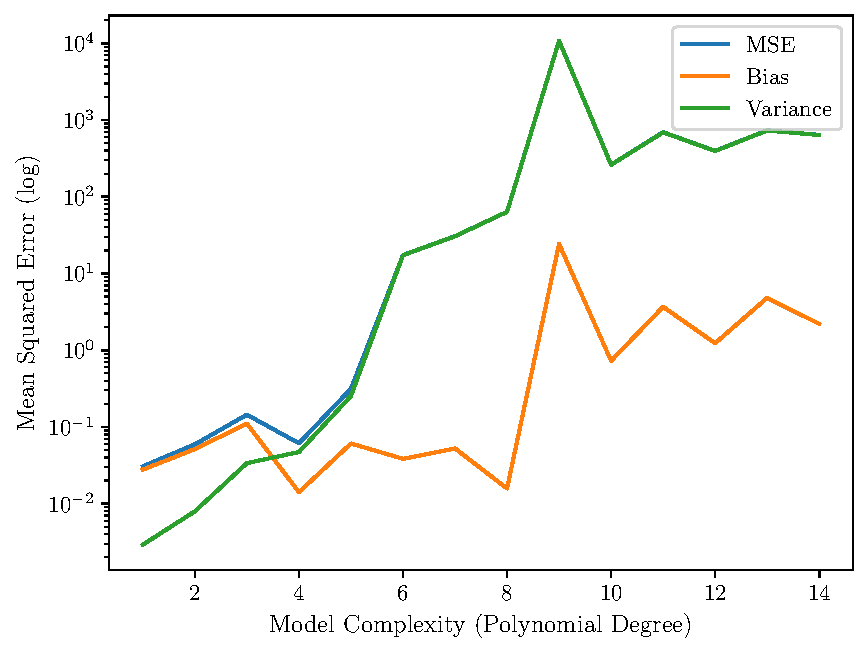
\includegraphics[width=0.9 \linewidth]{Figures/bias_variance_tradeoff.pdf}
    \caption{Bias Variance Tradeoff}
    \label{fig:BiasVariance1}
\end{figure}
Cool reference to the scikit api, \cite{sklearn_api}.


\begin{figure}[h]
    \centering
    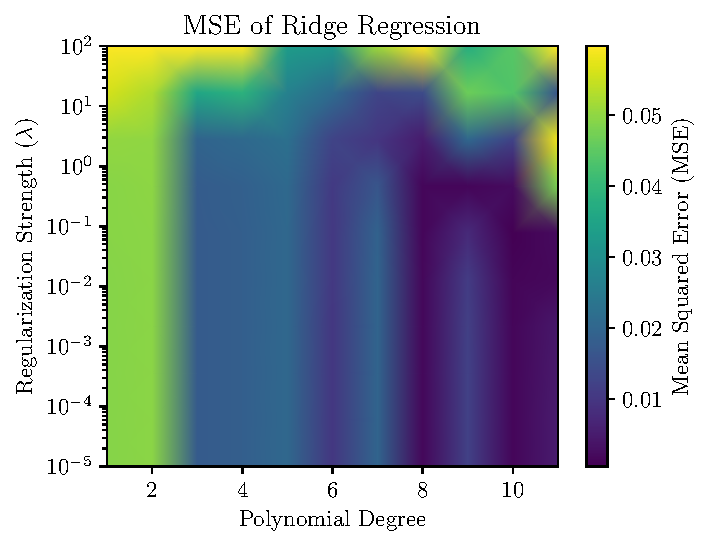
\includegraphics[width=0.9 \linewidth]{Figures/ridge_heatmap.pdf}
    \caption{Degree and Regularization Heatmap}
    \label{fig:DegRegHeat}
\end{figure}
The above heatmap, \ref{fig:DegRegHeat}, implies that a polynomial degree of 8 and a regularization value of slightly above $10^{-1} \lambda$ would be the best parameters for training the model.




\section{Conclusion}\label{section:conclusion} 

\begin{comment}
When you write the conclusion section you should focus on the following aspects:
\begin{itemize}
    \item State your main findings and interpretations
    \item Try to discuss the pros and cons of the methods and possible improvements
    \item State limitations of the study
    \item Try as far as possible to present perspectives for future work
\end{itemize}

\end{comment}

\bibliography{biblio}



\end{document}
